% Define document class
\documentclass[twocolumn]{aastex631}
\usepackage{showyourwork}

\newcommand{\sbu}{Department of Physics and Astronomy, Stony Brook University, Stony Brook NY 11794, USA}
\newcommand{\cca}{Center for Computational Astrophysics, Flatiron Institute, New York NY 10010, USA}

\usepackage{bbold}

% Begin!
\begin{document}

% Title
\title{Polka-dotted Stars: Mapping the Surface of HAT-P-11}

% Author list
\author[0000-0002-6650-3829]{Sabina Sagynbayeva}
\email{sabina.sagynbayeva@stonybrook.edu}
\affiliation{\sbu}
\affiliation{\cca}

\author[0000-0003-1540-8562]{Will M. Farr}
% \email{wfarr@flatironinstitute.org}
\affiliation{\sbu}
\affiliation{\cca}

\author[0000-0002-0296-3826]{Rodrigo Luger}
% \email{rodluger@gmail.com}
\affiliation{\cca}

% Abstract with filler text
\begin{abstract}
   
\end{abstract}

% Main body with filler text
\section{Introduction}
\label{sec:intro}
The quest to unravel the mysteries of distant planetary systems has led to a fast-evolving field of research, where exoplanet studies are at the forefront of 
astronomical investigations. Characterizing the surfaces of exoplanet-host stars is crucial for understanding the environments and evolution of their planetary 
systems. For example, the Sun's magnetic field drives the star's activity cycles, the heating of its outer atmosphere and the solar wind,
which affects the Earth's magnetosphere and biosphere \citep{Babcock1961,Charbonneau2014}. 
Therefore, constructing a catalogue of the magnetic properties of other stars similar to the Sun would support the quest towards understanding 
the population of detected exoplanets and the development of a highly generalizable theory on stellar magnetic dynamo.

The reverse statement is also true. The exisiting popultion of exoplanets along with their orbital parameters can help characterize their host-stars
in terms of their surface magnetic activity. Stellar surface features like spots and flares impact observables in planet-detection research including photometric 
variability, spectral line profiles, and radial velocity shifts. However, directly resolving stellar surfaces remains challenging.

While high-resolution spectroscopy provides the most robust method of determining stellar parameters, obtaining such data for large samples remains 
observationally expensive. Some recent works offered invaluable insights into the topographical characteristics of stars and their magnetic 
activity, responsible for the observed variatians on their surfaces. For example, the influence of star spots can be discerned through photometric 
data acquired from Kepler or TESS. \cite{Luger2021b} investigated the star spots features on the stellar surfaces using Gaussian Process (GPs) 
with a \emph{physically interpretable} kernel. They showed that it is hard to put constrains on star spot properties if you only have a light curve for 
one star, it is rather usefule though to perform the same analysis for an ensemble of stars. However, when a star has an exoplanet in orbit, 
the spot features become observable in the transit data, providing valuable constraints on the properties of these spots 
(whether they are dark or bright, their sizes, and their latitudes).

Data-driven approaches like Gaussian processes (GPs) offer pathways to map the surfaces of exoplanet hosts through measurable disk-integrated signals. 
In this work, we develop a Gaussian process framework to model the surfaces of exoplanet-host stars based on time-series photometry. We utilize 
expressive kernel function from \cite{Luger2021b}. We first use this model on a simulated data to test the model, then we apply the model to an active K-dwarf
HAT-P-11. 




%
\section{The Data}
The data is collected by the \emph{Kepler} mission and we extracted it using
\texttt{lightkurve}, a Python package for Kepler and TESS data analysis \citep{lightkurve}.
%
\begin{figure}[ht!]
    \script{TransitFitsWithStarry.py}
    \begin{centering}
        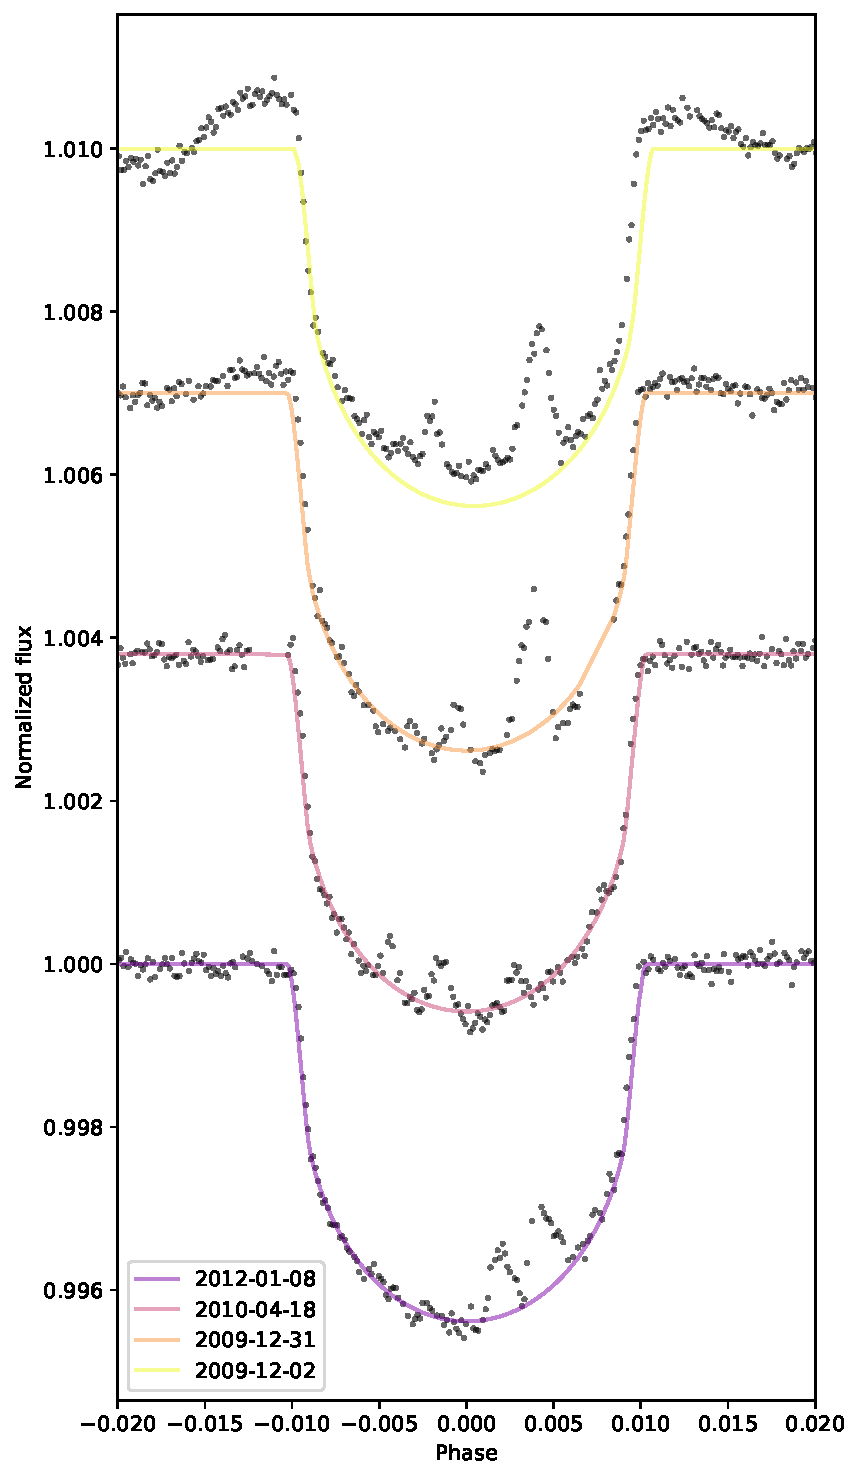
\includegraphics[width=\linewidth]{figures/TransitFitsWithStarry.pdf}
        \caption{
            Transit fits with starry -- no GPs.
        }
        \label{fig:TransitFitsStarry}
    \end{centering}
\end{figure}
%
\section{Hierarchical Bayesian model}

%
\subsection{The Model}
In this section, we will describe our Gaussian Process (GP) model and the likelihood calculation process used to estimate the model parameters. 

We solve for a large set of parameters that includes the GP hyperparameters, the star's and the planet's orbital parameters, respectively. 
\begin{linenomath}\begin{align}
    \label{eq:largetheta}
    \pmb{\Theta}
     & =
    \left(
    \theta_\bullet
    \,\,\,
    \theta_\star
    \,\,\,
    \theta_p
    \right)^\top
    \quad,
\end{align}\end{linenomath}

Separately, these parameters are defined as 
\begin{linenomath}\begin{align}
    \label{eq:thetastar}
    \pmb{\theta_\star}
     & =
    \left(
    i_\star
    \,\,\,
    m_\star
    \,\,\,
    u_1
    \,\,\,
    u_2
    \,\,\,
    P_\star
    \right)^\top
    \quad,
\end{align}\end{linenomath}
where $i_\star$ is the star's orbital inclination, $m_\star$ is the stellar mass in the units of the solar mass, $u_1$ and $u_2$ are limb-darkening coefficients,
and $P_\star$ is the rotational period of the star.

\begin{linenomath}\begin{align}
    \label{eq:thetap}
    \pmb{\theta_p}
     & =
    \left(
    i_p
    \,\,\,
    e
    \,\,\,
    \psi
    \,\,\,
    \omega
    \,\,\,
    P
    \,\,\,
    t_0
    \,\,\,
    R_p/R_\star
    \right)^\top
    \quad,
\end{align}\end{linenomath}
where $i_p$ is the planet's orbital inclination, $e$ is its eccenticity, $\psi$ is the stellar obliquity, $\omega$ is the argument of pericenter of the planet,
$P$ is the rotational period of the planet, $t_0$ is the transit start time, and $R_p/R_\star$ is the planet to star radius ratio.

We represent the GP hyperparameters as \emph{physically interesting} set of parameters $\pmb{\theta}_\bullet$ \citep{Luger2021b}:
%
\begin{linenomath}\begin{align}
        \label{eq:thetaspot}
        \pmb{\theta}_\bullet
         & =
        \left(
        n
        \,\,\,
        c
        \,\,\,
        \mu_\phi
        \,\,\,
        \sigma_\phi
        \,\,\,
        r
        \right)^\top
        \quad,
    \end{align}\end{linenomath}
%
where $n$ is the number of starspots, $c$ is their contrast (defined as the intensity difference between the spot and the 
background intensity, as a fraction of the background intensity),
$\mu_\phi$ and $\sigma_\phi$ are the mode and standard deviation
of the spot latitude distribution, respectively, and $r$ is the radius
of the spots.

We assume that the prior over $\mathbb{f}_{true}$ follows a multivariate Gaussian distribution, with a mean vector of zeros and a covariance 
matrix $\pmb{\Sigma}$. We use the quasi-periodic kernel to define the covariance matrix $\pmb{\Sigma}$, which is defined by \texttt{StarryProcess}.
We assume that the observations $\mathbb{f}_{obs}$ are corrupted by additive Gaussian noise, such that:
\begin{equation}
    \mathbb{f}_{obs} = \mathbb{f}_{true} + \epsilon
\end{equation}

where $\epsilon \sim \mathcal{N}(0, \sigma_n^2)$ is the noise term. Given the GP prior and the likelihood function, we can 
calculate the joint posterior distribution over the hyperparameters $\Theta$ and the true function $\mathbb{f}_{true}$ given the observed data $\mathbb{f}_{obs}$:
%
\begin{equation}
    p(\Theta, \mathbb{f}_{true} \mid \mathbb{f}_{obs}) \propto p(\Theta) p(\mathbb{f}_{true} \mid \Theta) p(\mathbb{f}_{obs} \mid \mathbb{f}_{true})
\end{equation}
%
where $P(\Theta)$ is the prior distribution over the hyperparameters, $P(\mathbb{f}_{true} \mid \Theta)$ is the likelihood of the true function given 
the hyperparameters, and $P(f_{obs} \mid f_{true})$ is the likelihood of the observed data given the true function.
We calculate the log-likelihood function, given by:
%
\begin{linenomath}\begin{align}
    \label{eq:log-likeSabina}
    \ln p(\mathbb{f}_{obs} \mid \pmb{\Theta}) 
    =
    & -\frac{1}{2} (\mathbb{f}_{obs} - \pmb{\mu})^T \pmb{\Sigma}^{-1} (\mathbb{f}_{obs} - \pmb{\mu}) 
    \nonumber       \\[0.75em]
    & -
    \frac{1}{2} \ln |\pmb{\Sigma}| - \frac{n}{2} \ln (2\pi)
    \quad,
\end{align}\end{linenomath}
%
or, as defined in eq. 14 of \citep{Luger2021}:
%
\begin{linenomath}\begin{align}
    \label{eq:log-likeRodrigo}
    \ln \mathcal{L}_m\left(\Theta\right)
    =
     & -\frac{1}{2}
    \mathbf{r}_m^\top\left(\Theta\right)
    \big[
        \pmb{\Sigma}\left(\Theta\right)
        \big]^{-1}
    \mathbf{r}_m\left(\Theta\right)
    \nonumber       \\[0.75em]
     & -
    \frac{1}{2}
    \ln \Big|
    \pmb{\Sigma}\left(\Theta\right)
    \Big|
    -
    \frac{K}{2}
    \ln \left( 2 \pi \right)
    \quad,
\end{align}\end{linenomath}
%
where
%
\begin{linenomath}\begin{align}
        \mathbf{r}_m\left(\pmb{\Theta}\right)
         & \equiv
        \mathbf{f}_m - \pmb{\mu}\left(\pmb{\Theta}\right)
    \end{align}\end{linenomath}
%
is defined as the residual vector,
%
$\Sigma$ is the full covariance, which is defined as 
%
\begin{linenomath}\begin{align}
    \pmb{\Sigma}\left(\Theta\right)
     & \equiv
    \pmb{\Sigma_y} + \pmb{\Sigma_d}
\end{align}\end{linenomath}
%
where $\pmb{\Sigma_y}$ is the covariance of the distribution over spherical harmonic coefficient
vectors $\mathbb{y}$, and $\pmb{\Sigma_d}$ is the data covariance, which is a diagonal
matrix whose entries are the squared uncertainty $\sigma_m^2$ corresponding to each data point in the light curve.
$| \cdots |$ denotes the determinant, and $K$ is the number of data points in
each light curve.%

For faster calculations we rewrite the likelihood function using \emph{the matrix conversion lemma}, also known as 
Woodbury-Sherman-Morrison identity (see e.g. \cite{Hogg2020}).


\section{Experiments}
In this section, we describe the experiments we did on synthetic light curves before going ahead and modeling the real data. The synthetic light curves were 
generated by initializing a planet and a star of similar parameters as HAT-P-11 b and HAT-P-11 have using \texttt{starry}. Then we draw \texttt{StarryProcess} 
samples from a prior to get spherical harmonic coefficients and consequently the simulated flux. 

\subsection{The issue of the normalization of light curves and units}
Before going on discussing the experiments produced for this paper, we first need to remind the reader of a subtlety of the flux normalization when we are given
the raw light curves from telescopes. The problem and the ways to tackle it were described in \cite{Luger2021a} and \cite{Luger2021b}. 

Briefly, the problem of normalization of light curves is related to the fact that the observed flux from a star can vary due to a variety of factors 
such as atmospheric effects, instrumental noise, and changes in the intrinsic brightness of the star itself. These variations can make it difficult 
to compare light curves of different stars or even the same star observed at different times. To address this problem, astronomers typically normalize 
light curves by dividing the observed flux by some factor (the median or mean of the flux) that is assumed to be constant over time. 
However, as was described in \cite{Luger2021a}, if a star has a single large equatorial spot of contrast $c$ viewed at some high inclination 
(\cite{Luger2021a} used the value of $60^o$), and another star with a spot at the same location but with half the contrast \emph{and} a large polar spot of 
comparable contrast, then the light curves for both of the stars become indistiguishable in the relative units astronomers observe them. In addition to normalizing 
the flux, \cite{Luger2021a} also added a \emph{baseline} (1 in their case), which is the flux one would have gotten from a spotless star, 
and is an additive component to the $Y_m^l$.

In our experiments, we noticed that dividing by a constant factor \emph{and} adding an additive baseline messes up the units due to the 
intricate transition between the spherical harmonics and flux unit bases. To address this issue, we opt for an alternative approach, wherein we 
impose a constraint upon the constant terms within the map, which correspond to a featureless star. Specifically, we achieve this by setting the prior distribution 
over these constant terms to be entirely uniform, thereby setting the first row of the precision matrix to zero.

% In our experiments, we noticed that dividing by a constant factor \emph{and} adding an additive baseline messes up the units due to the complex change of 
% basis from spherical harmonics to the flux units. Instead, in our model, we set the baseline, i.e the first column of the design matrix, $\pmb{\mathcal{A}}$, 
% to have the coefficients of the 0th harmonic, $Y^0_0$ -- the featureless star. Then, the normalization "factor" becomes additive (not multiplicative!). We're reminding 
% the reader that $\pmb{\mathcal{A}}$ covers the properties of the star and the planet (inclination, rotation period, transit, etc.), spherical harmonics desribe the
% properties of the starspots. Therefore, what we get is
% %
% \begin{linenomath}\begin{align}
%         \label{eq:fAy}
%         \mathbf{f} = \pmb{\mathcal{a}_0(t)} \mathbf{y_0(t)} + \sum_{l=1, m=-l}^{15} \pmb{\mathcal{a}_{lm}(t)} \mathbf{y_{lm}(t)},
%     \end{align}\end{linenomath}
% %
% where $\pmb{\mathcal{a}_0}$ is a column of $\pmb{\mathcal{A}}(I, P, \mathbf{u})$, which is the design matrix as a function of the stellar inclination, rotation period, 
% and limb-darkening coefficients; $\mathbf{y}$ is a spherical harmonic coefficient vector, and we define $\pmb{\mathcal{a}_0} \mathbf{y_0} = \pmb{m}$ 
% as the normalization constant, or a \emph{baseline}. We explicitly solve for the baseline in our model. Note that it is not constant with time due to the transits --
% $\pmb{m}$ drops when the planet is transitting the star.


\subsection{Short light curve}
For our initial experiment with minimal complexity, we created a synthetic light curve that involved a single planetary transit (therefore, 
\emph{a short light curve}). Here, we examined two distinct sampling techniques: No-U-Turn Sampling (NUTS) using \texttt{pymc3} and Markov Chain Monte Carlo (MCMC) 
using \texttt{emcee}. The MCMC technique exhibited a faster convergence rate of the walkers, despite the fact that it still required a significant amount of time.
\subsection{Long light curves (multiple transits)}
\section{Results and Discussion}

\bibliography{bib}

\end{document}
